\chapter{Precoding for SU-MIMO systems}
\label{chapter:precoding_for_su_mimo}

\section{Capacity Achieving Precoding}
\label{section:capacity_achieving_precoding}

Consider the \ac{SU}-\ac{MIMO} system model introduced in Section~\ref{subsection:su_mimo_system_model} together with the associated capacity optimization problem in \eqref{eq:capacity_su_mimo_gaussian_channel_optimization_problem}.
We first derive a more explicit expression for the channel capacity and then show that this capacity can be achieved by means of linear precoding.
The section follows a similar structure as in Chapter 3 of~\cite{cornelis_2025}.

\subsection{SU-MIMO Capacity}
\label{subsection:su_mimo_capacity}

The \ac{SVD} (see Appendix~\ref{appendix:svd}) of the channel matrix yields
\begin{equation}
\label{eq:svd_channel_matrix}
    \mathbf{H} = \mathbf{U} \boldsymbol{\Sigma} \mathbf{V}^H,
\end{equation}
where $\mathbf{U} \in \mathbb{C}^{N_R \times N_R}$ and $\mathbf{V} \in \mathbb{C}^{N_T \times N_T}$ are unitary matrices, and $\mathbf{\Sigma} \in \mathbb{R}^{N_R \times N_T}$ is a rectangular diagonal matrix which contains the singular values of $\mathbf{H}$ on its main diagonal in decreasing order.
The columns of $\mathbf{U}$ and $\mathbf{V}$ are contain the left and right singular vectors of $\mathbf{H}$, respectively.

Now define the transformed variables $\tilde{\mathbf{y}} = \mathbf{U}^H \mathbf{y}$, $\tilde{\mathbf{x}} = \mathbf{V}^H \mathbf{x}$, and $\tilde{\mathbf{n}} = \mathbf{U}^H \mathbf{n}$.
Since multiplication by a unitary matrix preserves the distribution of \ac{CS} complex Gaussian noise, $\tilde{\mathbf{n}}$ has the same distribution as $\mathbf{n}$. 
Moreover, because $\mathbf{U}$ and $\mathbf{V}$ are unitary, the transformations between $(\mathbf{x},\mathbf{y})$ and $(\tilde{\mathbf{x}},\tilde{\mathbf{y}})$ are bijective. 
The original channel can therefore be represented equivalently as
\begin{comment}
\begin{subequations}
\label{eq:su_mimo_equivalent_io_extended}
\begin{align}
    & \mathbf{y} = \mathbf{H} \mathbf{x} + \mathbf{n} \\
    & \Leftrightarrow \quad \mathbf{y} = \mathbf{U} \mathbf{\Sigma} \mathbf{V}^H \, \mathbf{x} + \mathbf{n} \\
    & \Leftrightarrow \quad \mathbf{U} \tilde{\mathbf{y}} = \mathbf{U} \mathbf{\Sigma} \mathbf{V}^H \, \mathbf{V} \tilde{\mathbf{x}} + \mathbf{n} \\
    & \Leftrightarrow \quad \tilde{\mathbf{y}} = \mathbf{U}^H \mathbf{U} \mathbf{\Sigma} \mathbf{V}^H \mathbf{V} \, \tilde{\mathbf{x}} + \mathbf{U}^H \mathbf{n} \\
    & \Leftrightarrow \quad \tilde{\mathbf{y}} = \mathbf{\Sigma} \tilde{\mathbf{x}} + \tilde{\mathbf{n}}.
\end{align}
\end{subequations}
\end{comment}
\begin{equation}
\label{eq:su_mimo_equivalent_io}
    \tilde{\mathbf{y}} = \mathbf{\Sigma}\tilde{\mathbf{x}} + \tilde{\mathbf{n}},
\end{equation}
which is obtained by applying the \ac{SVD} of the channel matrix and performing a change of variables. 
The channel in~\eqref{eq:su_mimo_equivalent_io} is equivalent to the original channel~\eqref{eq:su_mimo_io} in the sense that the transformation preserves the mutual information between input and output. Consequently, both channels have the same capacity.

The channel matrix $\mathbf{H}$ has exactly as many non-zero singular values $\{\sqrt{\sigma_i}\}$ as its rank, denoted as $R_H$.
Written component-wise, the equivalent channel becomes
\begin{equation}
\label{eq:su_mimo_equivalent_io_component_wise}
    \tilde{y}_i = \sqrt{\sigma_i} \, \tilde{x}_i + \tilde{n}_i \qquad \text{for} \quad i = 1, \dots, R_H,
\end{equation}
with $\tilde{y}_i = \tilde{n}_i$ for $i > R_H$. 
The equivalent channel decomposes into $R_H$ independent parallel scalar Gaussian subchannels, each with its own channel gain $\sqrt{\sigma_i}$. These subchannels and their gains are referred to as eigen subchannels and eigenmodes, respectively.
Since the components $\tilde{x}_i$ for $i > R_H$ have no effect on the output, they carry no information and can be set to zero.

For each eigen subchannel, the \acf{MI} is maximised by a zero-mean, \ac{CS} complex Gaussian input~\cite{telatar_1999}. Under this choice, the optimisation problem \eqref{eq:capacity_su_mimo_gaussian_channel_optimization_problem} simplifies to
\begin{equation}
\label{eq:capacity_su_mimo_gaussian_channel_optimization_problem_simplified}
\begin{aligned}
    & C = \max_{\{\mathbb{E}\left[|\tilde{x}_i|^2\right] \, \}} \; \sum_{i=1}^{R_H} \log_2\!\left(1 + \mathbb{E}\left[|\tilde{x}_i|^2\right] \, \frac{\sigma_i}{N_0} \right) \\
    & \text{s.t.} \quad \sum_{i=1}^{R_H} \mathbb{E}\left[|\tilde{x}_i|^2\right] \leq P_t.
\end{aligned}
\end{equation}

This maximization problem is solved using the Lagrange multiplier method (see Appendix~\ref{appendix:lagrange}).
The variances of the channel input need to be chosen according to the waterfilling principle~\cite{gallager_1968}:
\begin{equation}
    \mathbb{E}\left[\left\|\tilde{x}_i\right\|^2\right] = \left(\mu_{\text{w}} - \frac{N_0}{\sigma_i}\right)^{+},
\end{equation}
where the water level $\mu_{\text{w}}$ is found iteratively to satisfy the transmit power constraint with equality.

The resulting capacity is given by
\begin{equation}
\label{eq:capacity_su_mimo_gaussian_channel}
    C = \sum_{i=1}^{R_H} \, \log_2\!\left( \max(1, \, \mu_{\text{w}} \frac{\sigma_i}{N_0}) \right).
\end{equation}

\subsection{Optimal Precoder Design}
\label{subsection:optimal_precoder_design}

In this section, we design a linear precoder and combiner that achieve the capacity of the \ac{SU}-\ac{MIMO} channel.
We assume that the data symbol vector is \ac{CS} complex Gaussian distributed and spatially uncorrelated, and restrict ourselves to the case where the number of transmission streams equals the rank of the channel matrix.

% prove F and G achieve capacity by construction
For an arbitrary precoding matrix $\mathbf{F}$ and combining matrix $\mathbf{G}$, the data processing inequality~\cite{cover_thomas_2005} yields $I(\mathbf{x}; \mathbf{y}) \geq I(\mathbf{a}; \mathbf{z})$, where the \ac{MI} between the transmitted data symbols $\mathbf{a}$ and the decision variables $\mathbf{z}$ is given by:
\begin{subequations}
\label{eq:mi_az}
\begin{align}
    I(\mathbf{a}; \mathbf{z}) 
    &= \log_2\!\left(\det\!\left(\mathbf{I}_{N_s} + (\mathbf{G} \, \mathbf{C}_{\mathrm{n}} \, \mathbf{G}^H)^{-1} \, (\mathbf{G} \mathbf{H} \mathbf{F}) \, \mathbf{C}_{\mathrm{a}} \, (\mathbf{G} \mathbf{H} \mathbf{F})^H\right)\right) \label{eq:mi_az_a} \\
    &= \log_2\!\left(\det\!\left(\mathbf{I}_{N_s} + \tfrac{1}{N_0}(\mathbf{G} \mathbf{G}^H)^{-1} \, (\mathbf{G} \mathbf{H} \mathbf{F}) \, (\mathbf{G} \mathbf{H} \mathbf{F})^H\right)\right) \label{eq:mi_az_b}.
\end{align}
\end{subequations}
Expression~\eqref{eq:mi_az_a} follows directly from~\eqref{eq:mi_su_mimo_gaussian_channel} and the structural similarity between~\eqref{eq:su_mimo_io} and~\eqref{eq:su_mimo_precoding_combining_io}.
Expression~\eqref{eq:mi_az_b} then follows from~\eqref{eq:mi_az_a} upon substituting $\mathbf{C}_{\mathrm{a}} = \mathbf{I}_{N_s}$ and $\mathbf{C}_{\mathrm{n}} = N_0 \mathbf{I}$.

Motivated by the capacity derivation in the previous subsection~\ref{subsection:su_mimo_capacity}, we choose the columns of $\mathbf{F}$ and the rows of $\mathbf{G}$ as the $N_s$ most dominant right and left singular vectors of $\mathbf{H}$, respectively.
Since $N_s = R_H$, these are precisely the singular vectors associated with the non-zero singular values of $\mathbf{H}$.
In addition, the precoder incorporates the power allocation through a diagonal matrix $\mathbf{P}$.
More specifically, we set
\begin{equation}
\label{eq:su_mimo_optimal_precoder_and_combiner}
    \mathbf{F} = \mathbf{V}_{N_s} \, \sqrt{\mathbf{P}} \qquad \text{and} \qquad \mathbf{G} = \mathbf{U}_{N_s}^H.
\end{equation}

It follows from~\eqref{eq:su_mimo_optimal_precoder_and_combiner} that $I(\mathbf{a}; \mathbf{z}) = I(\mathbf{x}; \mathbf{y})$ for an appropriate choice of the power allocation $\mathbf{P}$.
This result can be verified in a brute-force way by substituting the particular precoder and combiner matrices from~\eqref{eq:su_mimo_optimal_precoder_and_combiner} into~\eqref{eq:mi_az} and replacing the channel matrix by its \ac{SVD} (see Appendix~\ref{appendix:calculations}).
\begin{comment}
\begin{subequations}
\begin{align}
    I(\mathbf{a}; \mathbf{z}) 
    &= \log_2\!\left(\det\!\left(\mathbf{I}_{N_s} + \tfrac{1}{N_0} (\mathbf{U}_{N_s}^H \mathbf{U}_{N_s})^{-1} \, (\mathbf{U}_{N_s}^H (\mathbf{U} \mathbf{\Sigma} \mathbf{V}^H) \mathbf{V}_{N_s} \sqrt{\mathbf{P}}) \, (\mathbf{U}_{N_s}^H (\mathbf{U} \mathbf{\Sigma} \mathbf{V}^H) \mathbf{V}_{N_s} \sqrt{\mathbf{P}})^H\right)\right) \\
    &= \log_2\!\left(\det\!\left(\mathbf{I}_{N_s} + \tfrac{1}{N_0} \mathbf{I}_{N_s} \, (\mathbf{U}_{N_s}^H \mathbf{U} \mathbf{\Sigma} \mathbf{V}^H \mathbf{V}_{N_s} \sqrt{\mathbf{P}}) \, (\mathbf{U}_{N_s}^H \mathbf{U} \mathbf{\Sigma} \mathbf{V}^H \mathbf{V}_{N_s} \sqrt{\mathbf{P}})^H\right)\right) \\
    &= \log_2\!\left(\det\!\left(\mathbf{I}_{N_s} + \tfrac{1}{N_0} \, \left(\begin{bmatrix} \mathbf{I}_{N_s} & \mathbf{0} \end{bmatrix} \, \begin{bmatrix} \mathbf{\Sigma}_{R_H} & \mathbf{0} \\ \mathbf{0} & \mathbf{0} \end{bmatrix} \, \begin{bmatrix} \mathbf{I}_{N_s} \\ \mathbf{0} \end{bmatrix} \sqrt{\mathbf{P}}\right) \, \left(\begin{bmatrix} \mathbf{I}_{N_s} & \mathbf{0} \end{bmatrix} \, \begin{bmatrix} \mathbf{\Sigma}_{R_H} & \mathbf{0} \\ \mathbf{0} & \mathbf{0} \end{bmatrix} \, \begin{bmatrix} \mathbf{I}_{N_s} \\ \mathbf{0} \end{bmatrix} \sqrt{\mathbf{P}}\right)^H\right)\right)  \\
    &= \log_2\!\left(\det\!\left(\mathbf{I}_{N_s} + \tfrac{1}{N_0} \, (\mathbf{\Sigma}_{N_s} \sqrt{\mathbf{P}}) \, (\mathbf{\Sigma}_{N_s} \sqrt{\mathbf{P}})^H\right)\right) \\
    &= \log_2\!\left(\det\!\left(\mathbf{I}_{N_s} + \tfrac{1}{N_0} \, \mathbf{\Sigma}_{N_s}^2 \, \mathbf{P}\right)\right) \\
    &= \log_2\!\left( \prod_{i=1}^{N_s} \left(1 + \frac{\sigma_i}{N_0}\, p_i \right) \right)  \\
    &= \sum_{i=1}^{N_s} \log_2\!\left(1 + \frac{\sigma_i}{N_0}\, p_i \right)
\end{align}
\label{eq:mi_az_equals_mi_xy}
\end{subequations}
\end{comment}
An alternative and more elegant approach consists in substituting the particular precoder and combiner into~\eqref{eq:su_mimo_precoding_combining_io} and comparing the resulting expression with the equivalent channel given in~\eqref{eq:su_mimo_equivalent_io}.
This yields
\begin{subequations}
\label{eq:su_mimo_optimal_precoding_combining_io}
\begin{align}
    \mathbf{z} &= \mathbf{U}_{N_s}^H \, \mathbf{U} \mathbf{\Sigma} \mathbf{V}^H \, \mathbf{V}_{N_s} \sqrt{\mathbf{P}} \, \mathbf{a} + \mathbf{U}_{N_s}^H \mathbf{n} \\
    %&= \begin{bmatrix} \mathbf{I}_{N_s} & \mathbf{0} \end{bmatrix} \; \begin{bmatrix} \mathbf{\Sigma}_{R_H} & \mathbf{0} \\ \mathbf{0} & \mathbf{0} \end{bmatrix} \; \begin{bmatrix} \mathbf{I}_{N_s} \\ \mathbf{0} \end{bmatrix} \; \sqrt{\mathbf{P}} \, \mathbf{a} + \tilde{\mathbf{n}} \\
    &= \mathbf{\Sigma}_{N_s} \, \sqrt{\mathbf{P}} \, \mathbf{a} + \tilde{\mathbf{n}},
\end{align}
\end{subequations}
where $\mathbf{\Sigma}_{N_s} \in \mathbb{R}^{N_s \times N_s}$ contains the $R_H$ non-zero singular values of $\mathbf{H}$ on its diagonal.

Comparing~\eqref{eq:su_mimo_optimal_precoding_combining_io} with~\eqref{eq:su_mimo_equivalent_io}, one can readily verify that $I(\mathbf{a}; \mathbf{z}) = I(\mathbf{x}; \mathbf{y})$, provided that the power allocated to each stream is set according to the waterfilling principle.
Hence, transmission with the precoder and combiner in~\eqref{eq:su_mimo_optimal_precoder_and_combiner} achieves the capacity of the \ac{SU}-\ac{MIMO} channel.
\bigskip

% interpretation optimal precoding scheme: decomposition
Denoting the $s$th element of the decision variable vector $\mathbf{z}$ by $z_s$, one can write~\eqref{eq:su_mimo_optimal_precoding_combining_io} component-wise as
\begin{equation}
\label{eq:su_mimo_optimal_precoding_combining_io_component_wise}
    z_s = \sqrt{\sigma_s} \, \sqrt{p_s} \, a_s + \tilde{n}_s \qquad \text{for} \quad s = 1, \dots, N_s.
\end{equation}

This expression shows that the precoder and combiner in \eqref{eq:su_mimo_optimal_precoder_and_combiner} diagonalize the \ac{SU}-\ac{MIMO} transfer matrix from~\eqref{eq:su_mimo_precoding_combining_io}.
The original \ac{SU}-\ac{MIMO} channel is decoupled into $N_s$ independent parallel scalar \ac{SISO} Gaussian subchannels with gains $\sqrt{\sigma_s}$, which coincides exactly with the decomposition of the equivalent channel in~\eqref{eq:su_mimo_equivalent_io_component_wise}.
A visualization of this decomposition is shown in Fig.~\ref{fig:su_mimo_channel_decomposition}.

As a result, the individual data streams become statistically independent. 
Detection therefore reduces to symbol-by-symbol processing rather than joint detection of the full decision-variable vector. 
This can lead to a significant reduction in receiver complexity, especially for systems with a large number of antennas and data streams.

\begin{figure}[htb]
    \centering

    \begin{subfigure}[c]{0.45\textwidth}
        \centering
        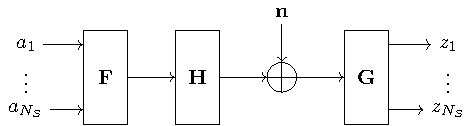
\includegraphics[width=\linewidth]
        {figures/background_material/03_su_mimo_precoding/out/channel_original.pdf}
        \caption{}
    \end{subfigure}
    \hfill
    \begin{subfigure}[c]{0.5\textwidth}
        \centering
        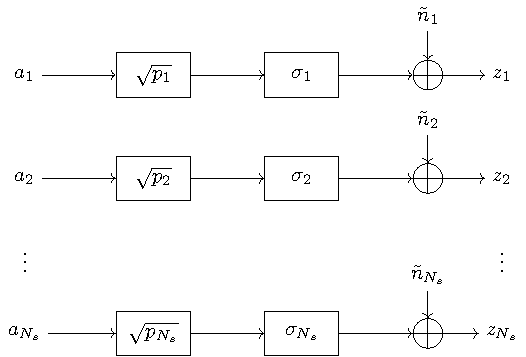
\includegraphics[width=\linewidth]
        {figures/background_material/03_su_mimo_precoding/out/channel_decomposition.pdf}
        \caption{}
    \end{subfigure}

    \caption[Decomposition of SU-MIMO Channel]
    {A block diagram of the original \ac{SU}-\ac{MIMO} channel (a) and its decomposition into parallel \ac{SISO} Gaussian eigen subchannels (b) by means of the optimal precoder and combiner.}

    \label{fig:su_mimo_channel_decomposition}
\end{figure}

% power allocation interpretation.
No general closed-form expression exists for the optimal water level, and hence for the resulting power allocation. Nevertheless, the optimal allocation is fully characterized by
\begin{equation}
\label{eq:_su_mimo_optimal_power_allocation}
    \sum_{i=1}^{N_s} p_i = P_t
    \qquad \text{and} \qquad
    p_i = \left(\mu_{\mathrm{w}} - \frac{N_0}{\sigma_i}\right)^+.
\end{equation}
Since the total allocated power is a monotonically increasing function of the water level $\mu_{\mathrm{w}}$, the latter can be determined numerically by means of a bisection method.
A more efficient approach exploits the fact that the number of active streams,
those receiving strictly positive power, is a discrete quantity.
First, the number of active streams is determined via a binary search in at most
$\lceil \log_2 N_s \rceil$ iterations, after which the water level follows in closed form.
Finally, the power allocated to each stream is computed.
The complete procedure is summarized in Algorithm~\ref{alg:waterfilling}.
Note that this approach relies on the fact that the set of candidate streams is finite and therefore does not extend in the same form to waterfilling algorithms for power allocation across the frequency spectrum of a frequency-selective channel.


% \section[Generalized Design of Linear Precoder and Combiner]{Generalized Design of Linear Precoder and Combiner using the WMMSE Criterion}

%\section{Maximum Information Rate Design}
